Neural style transfer (NST) methods manipulate images or videos to adapt to the visual characteristics of another image. NSTs are most commonly implemented through deep neural networks. The first publication using neural networks to perform NST was the work of Leon Gatys et al.\cite{DBLP:journals/corr/GatysEB15a} in 2015. This paper used a VGG19 architecture pre-trained on the ImageNet dataset. 


Just a year earlier, in 2014, Ian Goodfellow's groundbreaking Generative Adversarial Networks paper \cite{goodfellow2014generative}, proposed a new framework for estimating generative models using two, simpler models. Goodfellow's team was looking for an alternative to the, at the time, state-of-the-art undirected graphical models with latent variables such as restricted Boltzmann Machines \cite{computation_2021, rumelhart86a}. The main problem with this approach was that it was intractable for all but the most simple problems. The alternatives that did not involve defining a probability distribution explicitly, meaning that they could be trained by back-propagation, were in the form of generative stochastic networks\cite{DBLP:journals/corr/BengioT13}. This approach, however, still required Markov chains for sampling. Goodfellow's proposed Generative Adversarial Networks (GANs from now on) does away with the need for Markov chains for sampling, and because GANs do not require feedback loops during generation, they can leverage piecewise linear units and improve the backprop performance.

This "family" of networks has, over time, proven useful for NST. \emph{Style transfer} is a field that manipulates images or videos in order to apply the "style" or appearance of another image or video. Using GANs for style transfer was first explored by Tero Karras et al. in their paper: "A Style-Based Generator Architecture for Generative Adversarial Networks" \cite{stylegan}. An example of style transfer can be seen in Figure \ref{fig:style_ex}.

While GANs are on the bleeding edge regarding performance with NST, use cases with reduced computational capabilities might not take full advantage of them.


\begin{Figure}[h]
 \centering
 \includegraphics[width=\linewidth]{resources/style_example.png}
 \captionof{figure}{Style transfer examples}
 \label{fig:style_ex}
\end{Figure}


\section{Generative Adversarial Networks}
Goodfellow's approach was to use two models to solve the problem. The "generator" network generates candidates in the form of randomly sampled noise from true data distribution, while the "discriminator" network evaluates these samples. These two networks play a min-max game where the generator tries to generate "fake" samples that it thinks the discriminator will think are real, and "real" samples that it thinks the discriminator will think are fake, while the discriminator tries to "beat" the generator network by correctly classifying the incoming samples.
Over the years after Goodfellow's original GAN paper, the performance of these networks has improved quite a bit. Alec Radford's DCGANs\cite{radford_metz_chintala_2015} proposed the use of convolutional networks in place of fully connected networks, which improved the results and performance of the models. Further improvements for implementing GANs on large scale images such as Andrew Brock's 2018 \cite{DBLP:journals/corr/abs-1809-11096} paper on the subject, further proved that GANs could be used for larger resolution images.

\section{StyleGAN}

Tero Karras from NVIDIA proposed in 2018 an alternative GAN architecture to implement a style-transfer network.\cite{DBLP:journals/corr/abs-1912-04958} 

While the latent space code is provided to the generator network through its input layer, Karras omits it and starts from a pre-learned constant. 

NVIDIA's team provides their novel generator with a direct means to generate stochastic detail using explicit noise inputs, as single-channel images of uncorrelated Gaussian noise. These noise images are broadcasted to all feature maps using the learned per feature scaling factors and then added again to the output of their respective convolutions. 

Karras et al. had terrific results using this approach, as seen in Figure \ref{fig:style_face}.

\begin{Figure}[h]
 \centering
 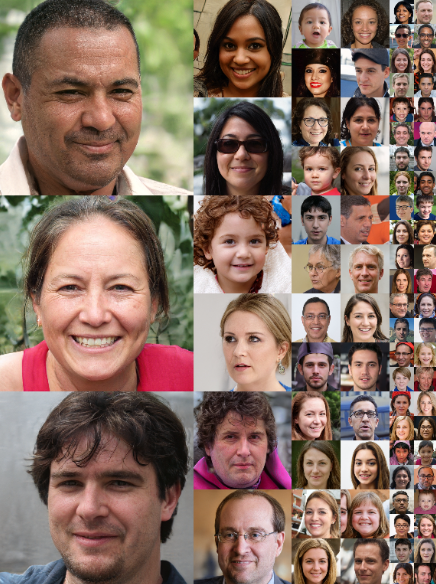
\includegraphics[width=8cm]{resources/styleface.png}
 \captionof{figure}{StyleGAN results}
 \label{fig:style_face}
\end{Figure}


In 2019, NVIDIA's team set out to improve StyleGAN by targeting several of it's characteristic artifacts\cite{DBLP:journals/corr/abs-1912-04958}. In this paper, the team sets out to redesign the generator normalization and regularize the generator to encourage good conditioning in the mapping from latent codes to images. 

To remove normalization artifacts, NVIDIA's team identifies an AdaIN operation that normalizes the mean and variance of every feature map separately, destroying any information found in the magnitudes of the features relative to each other. They instead remove the normalization step from the generator, causing the droplet artifacts to disappear.

On the other hand, the generator's architecture is revisited completely. The original StyleGAN applies bias and noise within the style block. 
This modification obtains more predictable results, moving these operations outside the style block and operating on normalized data. They also remove bias, noise, and normalization to the constant input without any observable drawback in performance or quality.

\subsection{StyleGAN2}
Later in 2020, Karras' team releases the "StyleGAN2" paper \cite{DBLP:journals/corr/abs-2006-06676}. This time around, Karras and his team set out to improve their StyleGAN to work with limited amounts of data. They propose implementing an adaptive discriminator augmentation mechanism that stabilizes training when the dataset used is small. They demonstrate that results are not greatly affected even without modifying the loss functions or the architecture of the network.